\chapter{工具实现与实验}\label{chapter_experiment}

\section{工具及其实现}

在上一章的方法中我们介绍了整体的优化框架一共分为4个不同的模块,分别是稳定性分析模块、计算路径提取模块、随机代数变换模块以及路径合并模块,在我们工具的实现中,每个模块都有对应的具体实现,其中路径提取模块以及随机代数变换模块存在一些技术难点,下面做具体介绍。

\subsection{基于KLEE符号执行的计算路径提取模块}

在这一模块中,我们通过符号执行的方式,将程序不稳定输入域上的计算路径提取出来。这一工作主要是基于符号执行技术来完成的,完全由自己手工来设计并实现一个符号执行工具将会是一项浩大的工程,因此我们选择对现有的符号执行工具进行改动,在其上添加新的功能以完成路径提取的工作。在这里我们选择KLEE作为我们的目标工具,KLEE本身是由斯坦福大学开发并发布的一个符号执行工具,其主要特点是能够通过符号执行的技术对复杂代码或者系统产生高覆盖率的测试用例。KLEE使用符号化的输入代替所有可能的具体的输入值,程序执行过程中的所有变量均会被表示成为关于这些符号化输入的表达式,并在遇到分支语句时构成对应路径的分支约束。从以上过程可以发现,KLEE能够完整的提供包括输入变量符号化,路径约束生产,符号执行等功能,因此我们选择在KLEE的基础上实现计算路径提取的功能。

然而,KLEE本身的功能并不完善,我们需要对KLEE进行改进以得到我们所需要的结果。我们主要对KLEE进行了以下改动,首先添加了对输出变量的识别功能,我们会在原数值计算程序中对需要输出的变量做类似于插桩的操作,将其标记为输出变量,表示我们需要在提取此变量关于程序输入的一个计算表达式,在KLEE的符号执行时,一旦遇到这样的变量,KLEE需要能够识别之,并在符号执行结束后在输出模块中将此变量对应的计算表达式输出。此外,我们的进行路径提取所得到的计算表达式中是必须能够包含一些基础的数学库函数的(比如sin、cos、ln函数等),然而KLEE在符号执行时却跳转入这些函数内部继续进行符号执行,这是我们不想看到的,为此,我们使KLEE在符号执行时有意的去忽略这些数学库函数,将其直接作为一个函数记录下来,而不是去做进一步的符号执行。最后是计算表达式的输出模块,在符号执行完成时,KLEE需要能够将需要的输出变量的计算表达式输出。

路径提取的结果最终会保存在一个路径文件中,对于如图\ref{lst:e_example_code}所示的使用泰勒级数近似计算自然对数e的数值计算程序,其对应抽取得到路径文件如图\ref{lst:e_example_pathfile}所示,路径文件中各个属性想详细解释见表\ref{tab:pathfile_attributes}。


\begin{figure}[thbp]
    \begin{lstlisting}[%
      xleftmargin=\columnsep,numberblanklines=true,boxpos=b,%,extendedchars=\true, %inputencoding=utf8%/latin1
      morekeywords={REAL, INTEGER}%keywords={main}
    ]
                REAL e_approx(INTEGER n) {
                    REAL z = 2; 
                    REAL y = 1;
                    for (INTEGER i = 0; i < n; ++i) {
                        y = y / i;
                        z = z + y;
                    }
                    return z;
                }
    
    \end{lstlisting}
    %\vspace*{-4mm}
    \caption{泰勒级数近似计算自然对数$e$程序代码}
    \label{lst:e_example_code}
    %\vspace*{-4mm}
\end{figure}


\begin{figure}[thbp]
\begin{lstlisting}[language=json,firstnumber=1]
{
    "program_name": "e_example",
    "function_name" : "e_approx",
    "variables" : {"n": "integer", "z": "decimal"},
    "input_variables": ["n"],
    "return": "z",
    "paths": [{
        "constrain": "true", 
        "path": ["procedure:p", "loop:l"]}],
    "loops": {
            "l": {
                "variables": {"i": "integer", "y": "decimal"},
                "initialize": {"i": "1", "y": "1.0"},
                "loop_body":[{
                    "constrain": "i<n",
                    "path": ["procedure:pp"],
                    "break": "false"
                    },
                    {
                    "constrain": "!(i<n)",
                    "path":[],
                    "break": "true"
                    }]
        }
    },
    "procedures": {
        "p": [["z", "1"]],
        "pp": [["y", "y/i"], ["z", "z+y"], ["i", "i+1"]]
    }
}
\end{lstlisting}
\caption{泰勒级数近似计算自然对数$e$程序路径文件}
\label{lst:e_example_pathfile}
\end{figure}

\begin{table}[!t]  
    \centering  
    \begin{tabular}{ll}  
      \\[-2mm]  
      \hline  
      \hline\\[-2mm]  
      {\bf \small 属性}  &   {\bf\small 含义}\\  
      \hline  
      \vspace{1mm}\\[-3mm]  
      program\_name     &   \tabincell{l}{程序名称}\\  
      \vspace{1mm}  
      function\_name    &   \tabincell{l}{函数名称}\\  
      \vspace{1mm}  
      variables         &   \tabincell{l}{所涉及到的变量及其对应类型}\\  
      \vspace{1mm}  
      intput\_variables &   \tabincell{l}{程序的输入变量}\\  
      \vspace{1mm}  
      output\_variables &   \tabincell{l}{程序的输出变量}\\  
      \vspace{1mm}  
      paths             &   \tabincell{l}{路径提取所得到的计算路径,为一个列表结构,列表中每个元素均为\\一个(约束,计算路径)二元组}\\  
      constrain         &   \tabincell{l}{计算路径对应的约束信息}\\  
      \vspace{1mm}  
      path              &   \tabincell{l}{一条计算路径,被抽象成为一个以procedure或是loop结构的列表的\\形式}\\  
      \vspace{1mm}  
      loops             &   \tabincell{l}{程序中涉及到的所有的循环信息}\\  
      \vspace{1mm}  
      loop\_body        &   \tabincell{l}{循环体信息,同样以计算路径的方式来表示,为一个列表结构,每个元\\素除了约束以及计算路径外,还附带了是否为循环出口的标记}\\  
      \vspace{1mm}  
      break             &   \tabincell{l}{循环体中的路径用来标记该路径是否为循环出口的标志}\\  
      \vspace{1mm}  
      procedures        &   \tabincell{l}{程序中所涉及到的所有的过程语句的信息,可以理解为顺序执行的一段\\代码,以列表形式给出,每个元素包含了变量及其对应计算形式信息}\\  
      \hline  
      \hline  
    \end{tabular}  
    \caption{路径文件属性说明}  
    \label{tab:pathfile_attributes}  
\end{table} 


\subsection{基于规则模板的随机代数变换引擎}

在前面的章节我们介绍了一个基于规则库的随机代数变换方法,来寻找一个不稳定计算过程的等价稳定计算形式。随机代数变换的核心是转换规则库,为了能够方便我们灵活的添加与删除规则,我们实现了一个随机代数变换引擎,规则库以模板文件的形式给出,我们可以非常容易地在规则库中添加新的规则。该随机代数变换引擎主要使用到了ANTLR(Another Tool for Language Recognition)库,该库是一个语法解析器的生成器,我们首先需要定义模板文件的语法,ANTLR可以自动地帮助我们生成该语法对应的解析器。该解析器解析规则模板文件能够得到每一条规则对应的语法树结构,在整个语法树结构上,我们去完成原始表达式形式的匹配,如果匹配成功,我们则将原始表达式转换成为对应的转换后的计算形式。

模板文件每一条规则的语法如下所示:

 \begin{gather*}
    \text{rule\_name} : \text{origin\_expr} \rightarrow \text{transformed\_expr} @ \text{constrain}
 \end{gather*}

 其中rule\_name表示规则名称,origin\_expr表示转换前的计算表达式,也就是需要我们进行匹配的计算表达式,transfromed\_expr表示转换后的计算表达式,constrain表示进行这样的转换需要满足的约束。表格\ref{tab:rule_list}列举了工具当前版本的模板文件中所实现的转换规则,如果我们后续需要添加新的转换规则,只需要在模板文件中添加即可。

\begin{table}[!t]  
    \centering  
    \scriptsize  
    \begin{tabular}{lc}  
      \\[-2mm]  
      \hline  
      \hline\\[-2mm]  
      {\bf \small Rule Name}  &   {\bf\small Content}\\  
      \hline  
      \vspace{1mm}\\[-3mm]  
      Negative     &   \tabincell{l}{$-A \leftrightarrow (-1) * A$}\\  
      \vspace{1mm}  
      Minus    &   \tabincell{l}{$A - B \leftrightarrow A + (-B)$}\\  
      \vspace{1mm}  
      Divide &   \tabincell{l}{$A / B \leftrightarrow A*(1/B)$}\\  
      \vspace{1mm}  
      CommutationPlus &   \tabincell{l}{$A + B \leftrightarrow B + A$}\\  
      \vspace{1mm}  
      CommutationMultiply &   \tabincell{l}{$A * B \leftrightarrow B * A$}\\  
      \vspace{1mm}  
      AssociationPlus &   \tabincell{l}{$A + B + C \leftrightarrow A + (B + C)$}\\  
      \vspace{1mm}  
      AssociationMultiply &   \tabincell{l}{$A * B * C \leftrightarrow A * (B * C)$}\\  
      \vspace{1mm}  
      Distribution1 &   \tabincell{l}{$A * (B + C) \leftrightarrow A * B + A * C$}\\  
      \vspace{1mm}  
      Distribution2 &   \tabincell{l}{$(A + B) * C) \leftrightarrow A * C + B * C$}\\  
      \vspace{1mm}  
      Distribution3 &   \tabincell{l}{$(A + B) / C) \leftrightarrow A / C + B / C$}\\  
      \vspace{1mm}  
      CommDenominator &   \tabincell{l}{$A/B+C/D \leftrightarrow (A*D+B*C)/(B*D)$}\\  
      \vspace{1mm}  
      FracReduction &   \tabincell{l}{$(A*N)/(B*N) \leftrightarrow A/(B)$}\\  
      \vspace{1mm}  
      NumeratorForm &   \tabincell{l}{$(A+B)/(C+D) \leftrightarrow (A+B)*(A-B)/((C+D)*(A-B))$}\\  
      \vspace{1mm}  
      DenominatorForm &   \tabincell{l}{$(A+B)/(C+D) \leftrightarrow (A+B)*(C-D)/((C+D)*(C-D))$}\\  
      \vspace{1mm}  
      Tan &   \tabincell{l}{$\tan(x) \leftrightarrow \sin(x)/\cos(x)$}\\  
      \vspace{1mm}  
      Sec &   \tabincell{l}{$\sec(x) \leftrightarrow 1/\cos(x)$}\\  
      \vspace{1mm}  
      Csc &   \tabincell{l}{$\csc(x) \leftrightarrow 1/\sin(x)$}\\  
      \vspace{1mm}  
      Cot &   \tabincell{l}{$\cot(x) \leftrightarrow \cos(x)/\sin(x)$}\\  
      \vspace{1mm}  
      SinPlus &   \tabincell{l}{$\sin(A+B) \leftrightarrow \sin(A)*cos(B)+cos(A)*\sin(B)$}\\  
      \vspace{1mm}  
      CosPlus &   \tabincell{l}{$\cos(A+B) \leftrightarrow \cos(A)*\cos(B)-\sin(A)*\sin(B)$}\\  
      \vspace{1mm}  
      TayporExp &   \tabincell{l}{$\text{sum}(k, 0, n, x\string^k/\text{\text{fac}}(k)) \leftrightarrow e\string^x$}\\  
      \vspace{1mm}  
      TaylorLn &   \tabincell{l}{$\text{sum}(k, 0, n, -x\string^k/k) \leftrightarrow \ln(1-x) @ \text{abs}(x) < 1$}\\  
      \vspace{1mm}  
      TaylorSin &   \tabincell{l}{$\text{sum}(k, 0, n, (-1)\string^k*x\string^(2*k+1)/\text{fac}(2*k+1)) \leftrightarrow \sin(x)$}\\  
      \vspace{1mm}  
      TaylorCos &   \tabincell{l}{$\text{sum}(k, 0, n, (-1)\string^k*x\string^(2*k)/\text{fac}(3*k)) \leftrightarrow \cos(x)$}\\  
      \vspace{1mm}  
      PolarRepresentation &   \tabincell{l}{$A+B*I \leftrightarrow sqrt(A\string^2+B\string^2)*e\string^(atan(B/A)*I)$}\\  
      \vspace{1mm}  
      Midarc &   \tabincell{l}{$(e\string^(I*a)+e\string^(I*b))/\text{abs}(e\string^(I*a)+e\string^(I*b)) \leftrightarrow e\string^(I*(a+b)/2)$}\\  
      \vspace{1mm}  
      StirlingGamma &   \tabincell{l}{$(X-0.5)*\ln(X)-X+\ln(2*pi)/2+\text{sum}(k, 1, n, \text{bnl}(2*k)/(2*k*(2*k-1)*X\string^(2*k-1))) \leftrightarrow \ln(\text{gamma}(X))$}\\  
      \vspace{1mm}  
      GammaTrans &   \tabincell{l}{$\text{gamma}(X) \leftrightarrow X*\text{gamma}(X-1)$}\\  
      \vspace{1mm}  
      Gamma\_0 &   \tabincell{l}{$\text{gamma}(X) \leftrightarrow 1/X+r @ \text{abs}(X) < \epsilon$}\\  
      \vspace{1mm}  
      Gamma\_1 &   \tabincell{l}{$\text{gamma}(X) \leftrightarrow r-1-1/(X+1) @ \text{abs}(X+1) < \epsilon$}\\  
      \vspace{1mm}  
      Gamma\_2 &   \tabincell{l}{$\text{gamma}(X) \leftrightarrow (8-4*r+3*X-2*r*X)/(4*X+8) @ \text{abs}(x+2) < \epsilon$}\\  
      \hline  
      \hline  
    \end{tabular}  
    \caption{转化规则模板文件中的转换规则}  
    \label{tab:rule_list}  
\end{table} 

\section{工具使用}

NGOpt工具在使用过程对用户非常友好,每一个模块的输出均会以文件的形式保存下来,用以提供给下一个模块作为输入使用,当想单独执行某几个模块时也可以选择性地执行,同时这样做也方便用户查看每个模块的中间结果。稳定性分析模块在执行结束后首先会生成一个json形式的以sa后缀结尾文件,里面存储了稳定性分析得到的结果,即原数值计算程序对应的稳定输入域,不稳定输入域信息。然后,路径提取模块对程序进行符号执行,提取程序的计算路径,将结果保存在一个以pth为后缀的路径文件中,具体形式上一小节已经作了具体介绍,在此不再赘述。紧接着,路径优化的模块会读取上个模块的输出,对其中的不稳定路径进行优化,得到的结果保存在opt.pth文件中,该文件结构与pth基本一致,只不过在文件中每条路径上新添加了具体的实现信息,以备后续路径合并时使用。最后,路径合并模块读取上一步的输出文件,将每条路径结合其实现信息组合成为最后的优化后程序。

在使用NGOpt之前,用户首先需要对工具进行一定的配置工作,所有的配置选项都保存在一个名为config.py的python文件中,下面对配置文件的选项做相关的介绍:

\begin{itemize}

    \item MODULES = all, sa, pe, st, pm 

    执行模块设置。用户可以在配置文件中制定需要执行的模块,包括了sa(stable analysis)代表稳定性分析模块,pe(path extraction)代表了路径提取模块,sat(stochastic algebraic transformation)随机代数变换模块,pm(path merge)代表了路径合并模块,每个模块之间使用","分隔,同时用户也可以使用all这个配置选项来选择执行所有的模块。需要注意的是,前后模块之间有依赖关系,必须确保每个模块都有对应的输入文件才能选择执行,例如执行sat模块必须保证上一个模块的输出pth文件存在才能够执行,否则程序会报错。

    \item ERROR\_TOLERANCE = 3E-14\%

    允许误差设置。该设置用于稳定性分析模块,代表了程序在进行稳定性分析时,能够所允许的任意精度程序与浮点精度程序在某一个输入域上的最大相对误差,超过这个误差,我们认为该输入域是不稳定的,若误差能够保证在这个范围以内,则我们认为该输入域为稳定的。IEEE754浮点数标准规定了,一个双精度浮点数由64个比特位组成,其中52位为有效数字位。因此,一个浮点数的基本表示误差在10-14\%左右。也就是说,就算我们仅仅对一个浮点数进行赋值操作,不考虑其他任何的计算操作,这样的赋值操作也有可能引入百分之1E-14的相对误差。因此我们一般将此设置项设置为3E-14\%,也就是说,当一个数值计算过程使用浮点数实现时,与其任意精度实现在某一输入域上的最大相对误差不超过3E-14\%时,我们便认为此输入域是稳定的。

    \item EXPR\_SETNUM = 100

    等价代数集合设置。该设置表示在进行随机代数变换时,我们产生的等价代数集合的最大大小,一旦达到该大小然而还未寻找到稳定的计算形式,我们则结束搜索的过程,使用原任意精度的数值计算过程。

    \item TIMEOUT = 10min

    随机代数变换超时设置。该设置表示在进行随机代数变换时,允许的最大搜索时间,一旦超时,我们同样的也会结束整个搜索过程,使用原任意精度的数值计算过程。

\end{itemize}

在完成了上述的相关配置后,用户便可以直接执行优化程序,将原程序代码的文件路径作为命令行参数给出,在完成优化后在同目录下会生成多个中间结果的文件,以及最终的优化后的以opt.cc结尾的代码文件。

\section{实验}

为了验证NGOpt在真实程序上的优化效果,我们进行了两部分实验:实验一的实验对象是iRRAM任意精度数值计算库的中典型的数值计算程序,进行了数值计算程序在优化前后的运行结果以及运行效率的对比。在实验二中,我们选取了gblic中一些常用的数学函数,我们自己实现了一套这些数学函数的任意精度版本,并使用我们的优化框架对其进行了优化,然后与glibc中的代码实现进行了一系列比较,主要为了研究我们的优化框架是否真的能够帮助软件开发人员开发易读易维护且正确高效的数值计算程序。

两次实验使用的电脑为Dell Workstation Precision T1700,处理器为Intel(R) Core(TM) i7-4790@3.60GHz 8核处理器,内存16GB,操作系统为Ubuntu 14.04LTS,使用系统默认编译器gcc4.8.0。

\subsection{iRRAM任意精度程序实验}

为了在版本迭代时能够方便地进行测试,iRRAM任意精度数值计算库的源码中附带了一系列数值计算程序,这些数值计算程序由任意精度编写,并且囊括了许多经典的数值计算问题。我们对这些程序进行了筛选,去除掉了一些与数值计算问题无关的测试程序(比如直接将一个字符串转换为数值类型的测试程序)选出了11个数值计算程序作为我们的优化目标,如表\ref{tab:irram_examples}所示。

\begin{table}[h]  
    \centering  
    \begin{tabular}{ll}  
      \\[-2mm]  
      \hline  
      \hline\\[-2mm]  
      {\bf \small 程序}  &   {\bf\small 说明}\\  
      \hline  
      \vspace{1mm}\\[-3mm]  
      analytic     &   \tabincell{l}{以一个简单算法计算$1/2^{20}$的计算程序}\\  
      \vspace{1mm}  
      e\_example    &   \tabincell{l}{使用级数$\sum_{i=0}^{n}1/i!$计算自然对数$e=2.71828...$}\\  
      \vspace{1mm}  
      float\_extension &   \tabincell{l}{计算$2+\sum_{i=1}^{100,000}1/\sqrt{i}$的数值计算程序}\\  
      \vspace{1mm}  
      gamma\_bernoulli &   \tabincell{l}{使用斯特林方法近似计算欧拉常数$\gamma = 0.577...$}\\  
      \vspace{1mm}  
      harmonic &   \tabincell{l}{计算调和级数的前$n$项和}\\  
      \vspace{1mm}  
      itsyst  & \\
      itsyst2 &   \tabincell{l}{以不同的输入迭代计算$x_{i+1} = 3.75x_i(1-x_i)$}\\  
      itsyst3 &  \\
      \vspace{1mm}  
      jmmuller &   \tabincell{l}{以不同输入迭代计算$x_{i+2}=3000/(1130-x_i(111-x_{i-1})$}\\  
      jmmuller2 &  \\
      \vspace{1mm}  
      lambov &   \tabincell{l}{计算泰勒余项}\\  
      \hline  
      \hline  
    \end{tabular}  
    \caption{iRRAM数值计算库中示例程序说明}  
    \label{tab:irram_examples}  
\end{table} 

对于每个计算程序,我们对比了以下三个不同版本的程序代码的运行结果以及运行效率:

\begin{itemize}
    \item {\kaishu 任意精度程序} \\
    这是iRRAM自带的程序,使用任意精度类型的实现。这个版本的数值计算程序能够保证绝对的正确性,并且在计算资源允许的情况下,对于每一个数值计算程序,其可以输出任意多位的有效数字。

    \item {\kaishu 直接的浮点精度程序} \\
    我们保持原任意精度的计算过程不变,将其中的变量的类型由任意精度转换成为普通的双精度浮点数类型,得到了这样的直接的浮点精度程序。

    \item {\kaishu 优化后程序} \\
    们将原任意精度程序作为输入,交给我们的优化工具NGOpt,得到的优化后程序。
\end{itemize}

实验一的实验结果如表\ref{fig:error_time}所示,从表格中我们能够清楚的看到,所有优化后的数值计算程序与原任意精度程序输出的相对误差均不超过$3E-14$,即我们优化后的程序都是计算稳定的,我们的优化过程能够保证程序的正确性。相比较而言,对于直接的浮点精度程序来说,其总体的平均相对误差达到了2.36E+03\%,唯有非常简单的计算$1/2^{20}$的数值计算程序与原任意精度程序的误差相对小。因此,我们可以得出结论,我们的优化框架能够保持程序本身的正确性,优化后的数值计算程序仍然是计算稳定的。

除了比较程序的运行结果,我们同时也比较了三种不同程序运行时间。从表中可以看到,原任意精度程序的平均运行时间为44.6秒,然而直接的浮点精度程序以及我们优化后的程序的平均运行时间分别为0.739秒和0.287秒。对比一下直接的浮点精度的运行时间与优化后程序的运行时间我们可以发现,有时是优化后程序运行时间较短,然而又有些时候则是直接的浮点精度程序运行地更快一些,这是由优化工具找到的等价计算过程的复杂程度决定的,有时候我们能够找到更加简单的计算过程,因此优化后程序的运行时间要比直接的浮点精度程序短。有时生成的优化后程序会非常的复杂,因此其运行时间会比直接的浮点精度程序稍长一些。从这些时间数据我们可以得出这样的结论,我们的优化工具能够在保证程序正确性的同时,大大提升程序的运行效率。

\begin{table*}[thbp]
   \centering
   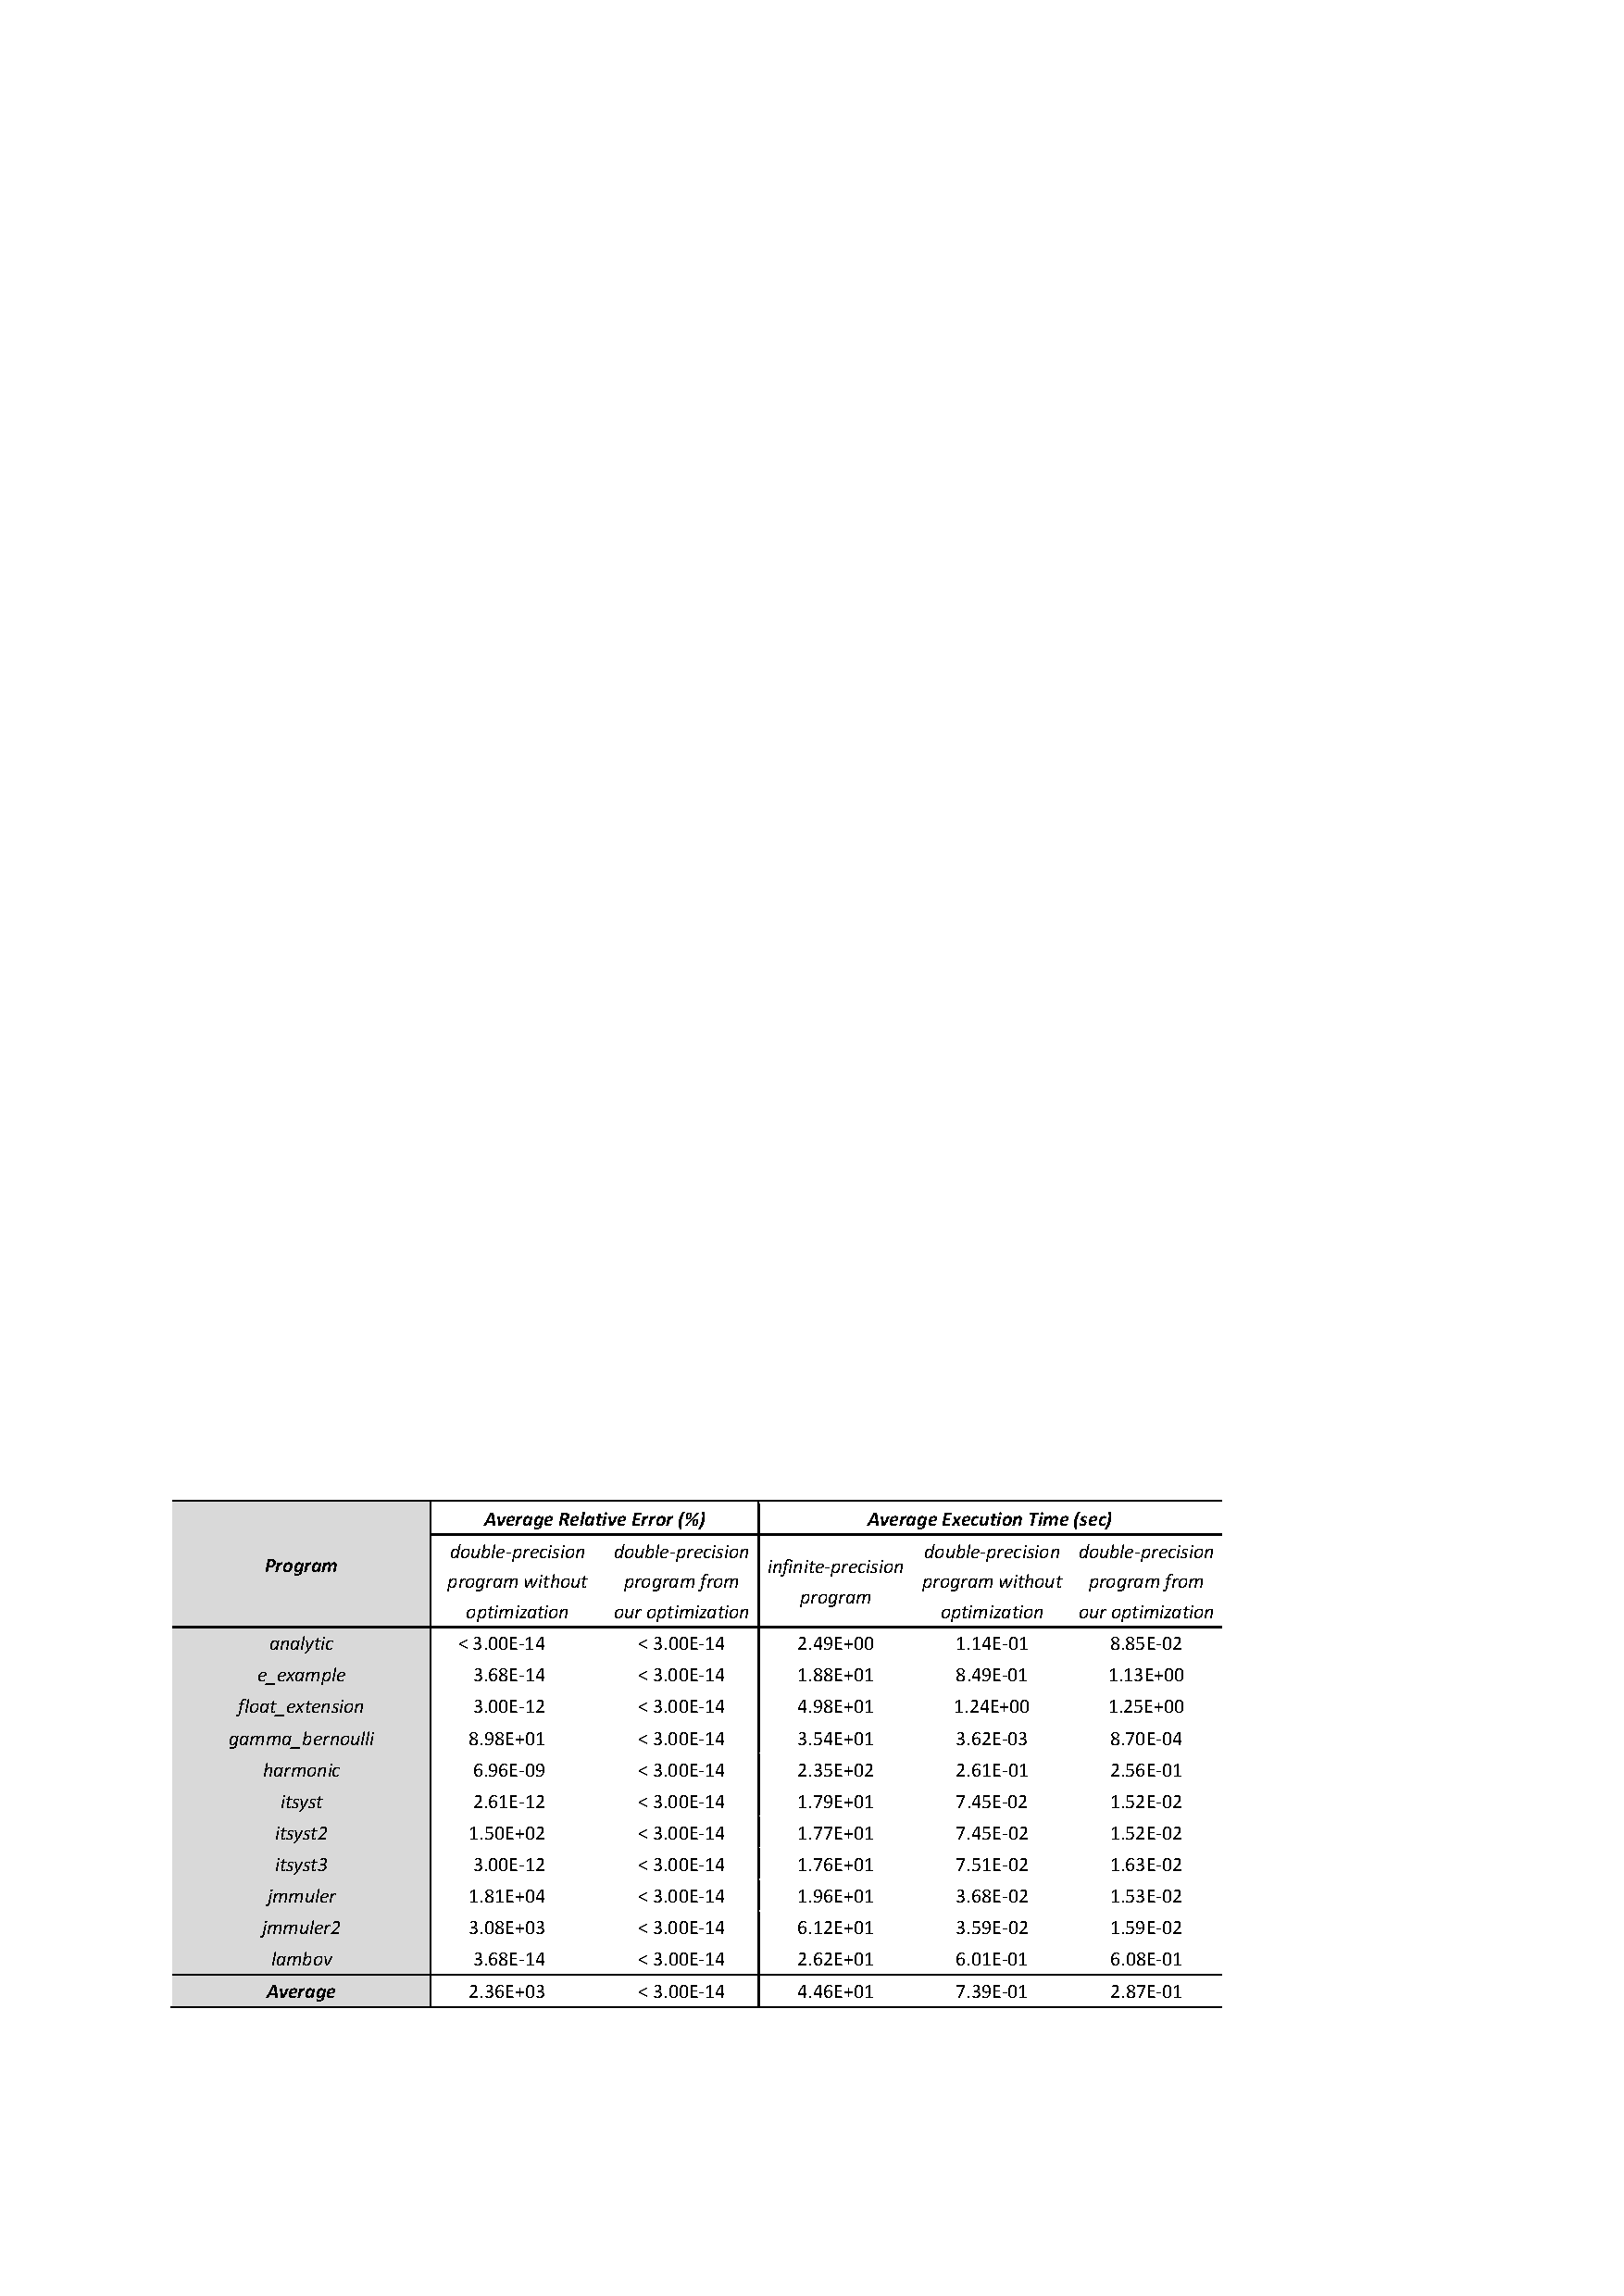
\includegraphics[width=\columnwidth]{fig/EvalTable_ErrorTime.pdf}
   \caption{iRRAM示例程序误差即运行时间表} \label{fig:error_time}
\end{table*}

\subsection{glibc数学函数库实验}

GNU C库是一个被广泛应用的C函数库,已有30年的历史,目前最主要的应用是配合Linux内核,是GNU/Linux操作系统的重要组成部分。在这个实验中,我们选取了GNU C库中部分常用的数据函数,使用任意精度对这些函数进行了重新实现,然后对这样的任意精度代码进行了优化,保证了优化后代码的正确性。然后,我们比较了这样重新实现的任意精度代码与原glibc中函数实现代码的一些可维护性指标,从而说明我们的优化工具能够帮助软件开发人员更加轻松地编写高可读性、可维护性并且正确高效的代码。

我们使用了业界常用的几种软件度量标准,包括了霍尔斯特德复杂度(Halstead Volume)、圈复杂度(Cyclomatic Complexity)以及可维护性指数(Maintainbility Index)。

霍尔斯特德复杂度是由霍尔斯特德在1977年提出的一种软件度量标准,其主要是依据程序源代码中的运算符和操作数来衡量源程序代码的复杂程度。在Halstead方法中,运算符是指用来处理程序中常量和变量的语法元素等,如算术运算符、逻辑运算符、关系运算符、流程控制语句、函数调用等;操作数则是指源程序代码中的常量和变量等,但对非执行语句,如注释,则不进行考虑。Halstead方法使用了以下4个基本测量数据:

\begin{itemize}
    \item 程序中运算符总数N1
    \item 程序中操作数总数N2
    \item 程序中运算符种类数n1
    \item 程序中操作数种类数n2
\end{itemize}

根据以上4个测量数据,可以在以下几个方面对源程序代码的复杂性进行度量:

\begin{itemize}
    \item 实际程序长度 N=N1+N2
    \item 编程语言层次 L=(2/n1)*(n2/N2)
    \item 程序容量 V=(N1+N2)*log2(n1+n2) 
    \item 预测程序长度 N'= n1*log2n1+n2*log2n2
    \item 估计程序工作量 E'=V/L=(n1*N2*(N1+N2)*log2(n1+n2))/(2*n2)
    \item 预测程序错误数E"=((N1+N2)*log2(n1+n2))/3000
\end{itemize}

在本次实验中,我们使用了程序容量V这一度量指标,这一指标代表了写一个程序所需的信息量,越高则表明该程序越难以开发和维护。

圈复杂度也被称作条件复杂度或是循环复杂度,是另一种代码复杂程度的衡量标准,是由 Thomas J. McCabezz,Sr. 在 1976 年提出,圈复杂度是对源代码中线性独立路径数的定量测量。

圈复杂度由程序的控制流图来计算,程序的控制流图是一个有向图,图中的节点为程序的基础模块,若一个模块结束后,可能会运行另一个模块,则用箭头链接二个模块,并标示可能的运行顺序。程序的圈复杂度由以下公式来计算:

\begin{align*}
    C = E - X + 2P
\end{align*}

其中 E 为图中边的个数, X 为图中节点的个数,P 为连接组件的个数。圈复杂度高说明程序代码的判断逻辑复杂,代码质量越低且更加难以测试和维护。

可维护性指数是一个结合了霍尔斯特德复杂度,圈复杂度以及代码行数的综合性指标,其计算公式如下所示:

\begin{align*}
    MI = 171 - 5.2\ln V - 0.23C - 16.2\ln LOC + 50\sin\sqrt{2.46CM}
\end{align*}

其中V代表了程序容量,C代表了程序圈复杂度,LOC代表了代码行数,CM代表了程序中的注释占总程序量的百分比,由于我们只考虑数学函数数值计算程序的具体代码实现,所以我们忽略计算公式中的CM。可维护性指数越低,表明程序越易于维护。

\begin{table*}[thbp]
    \centering
    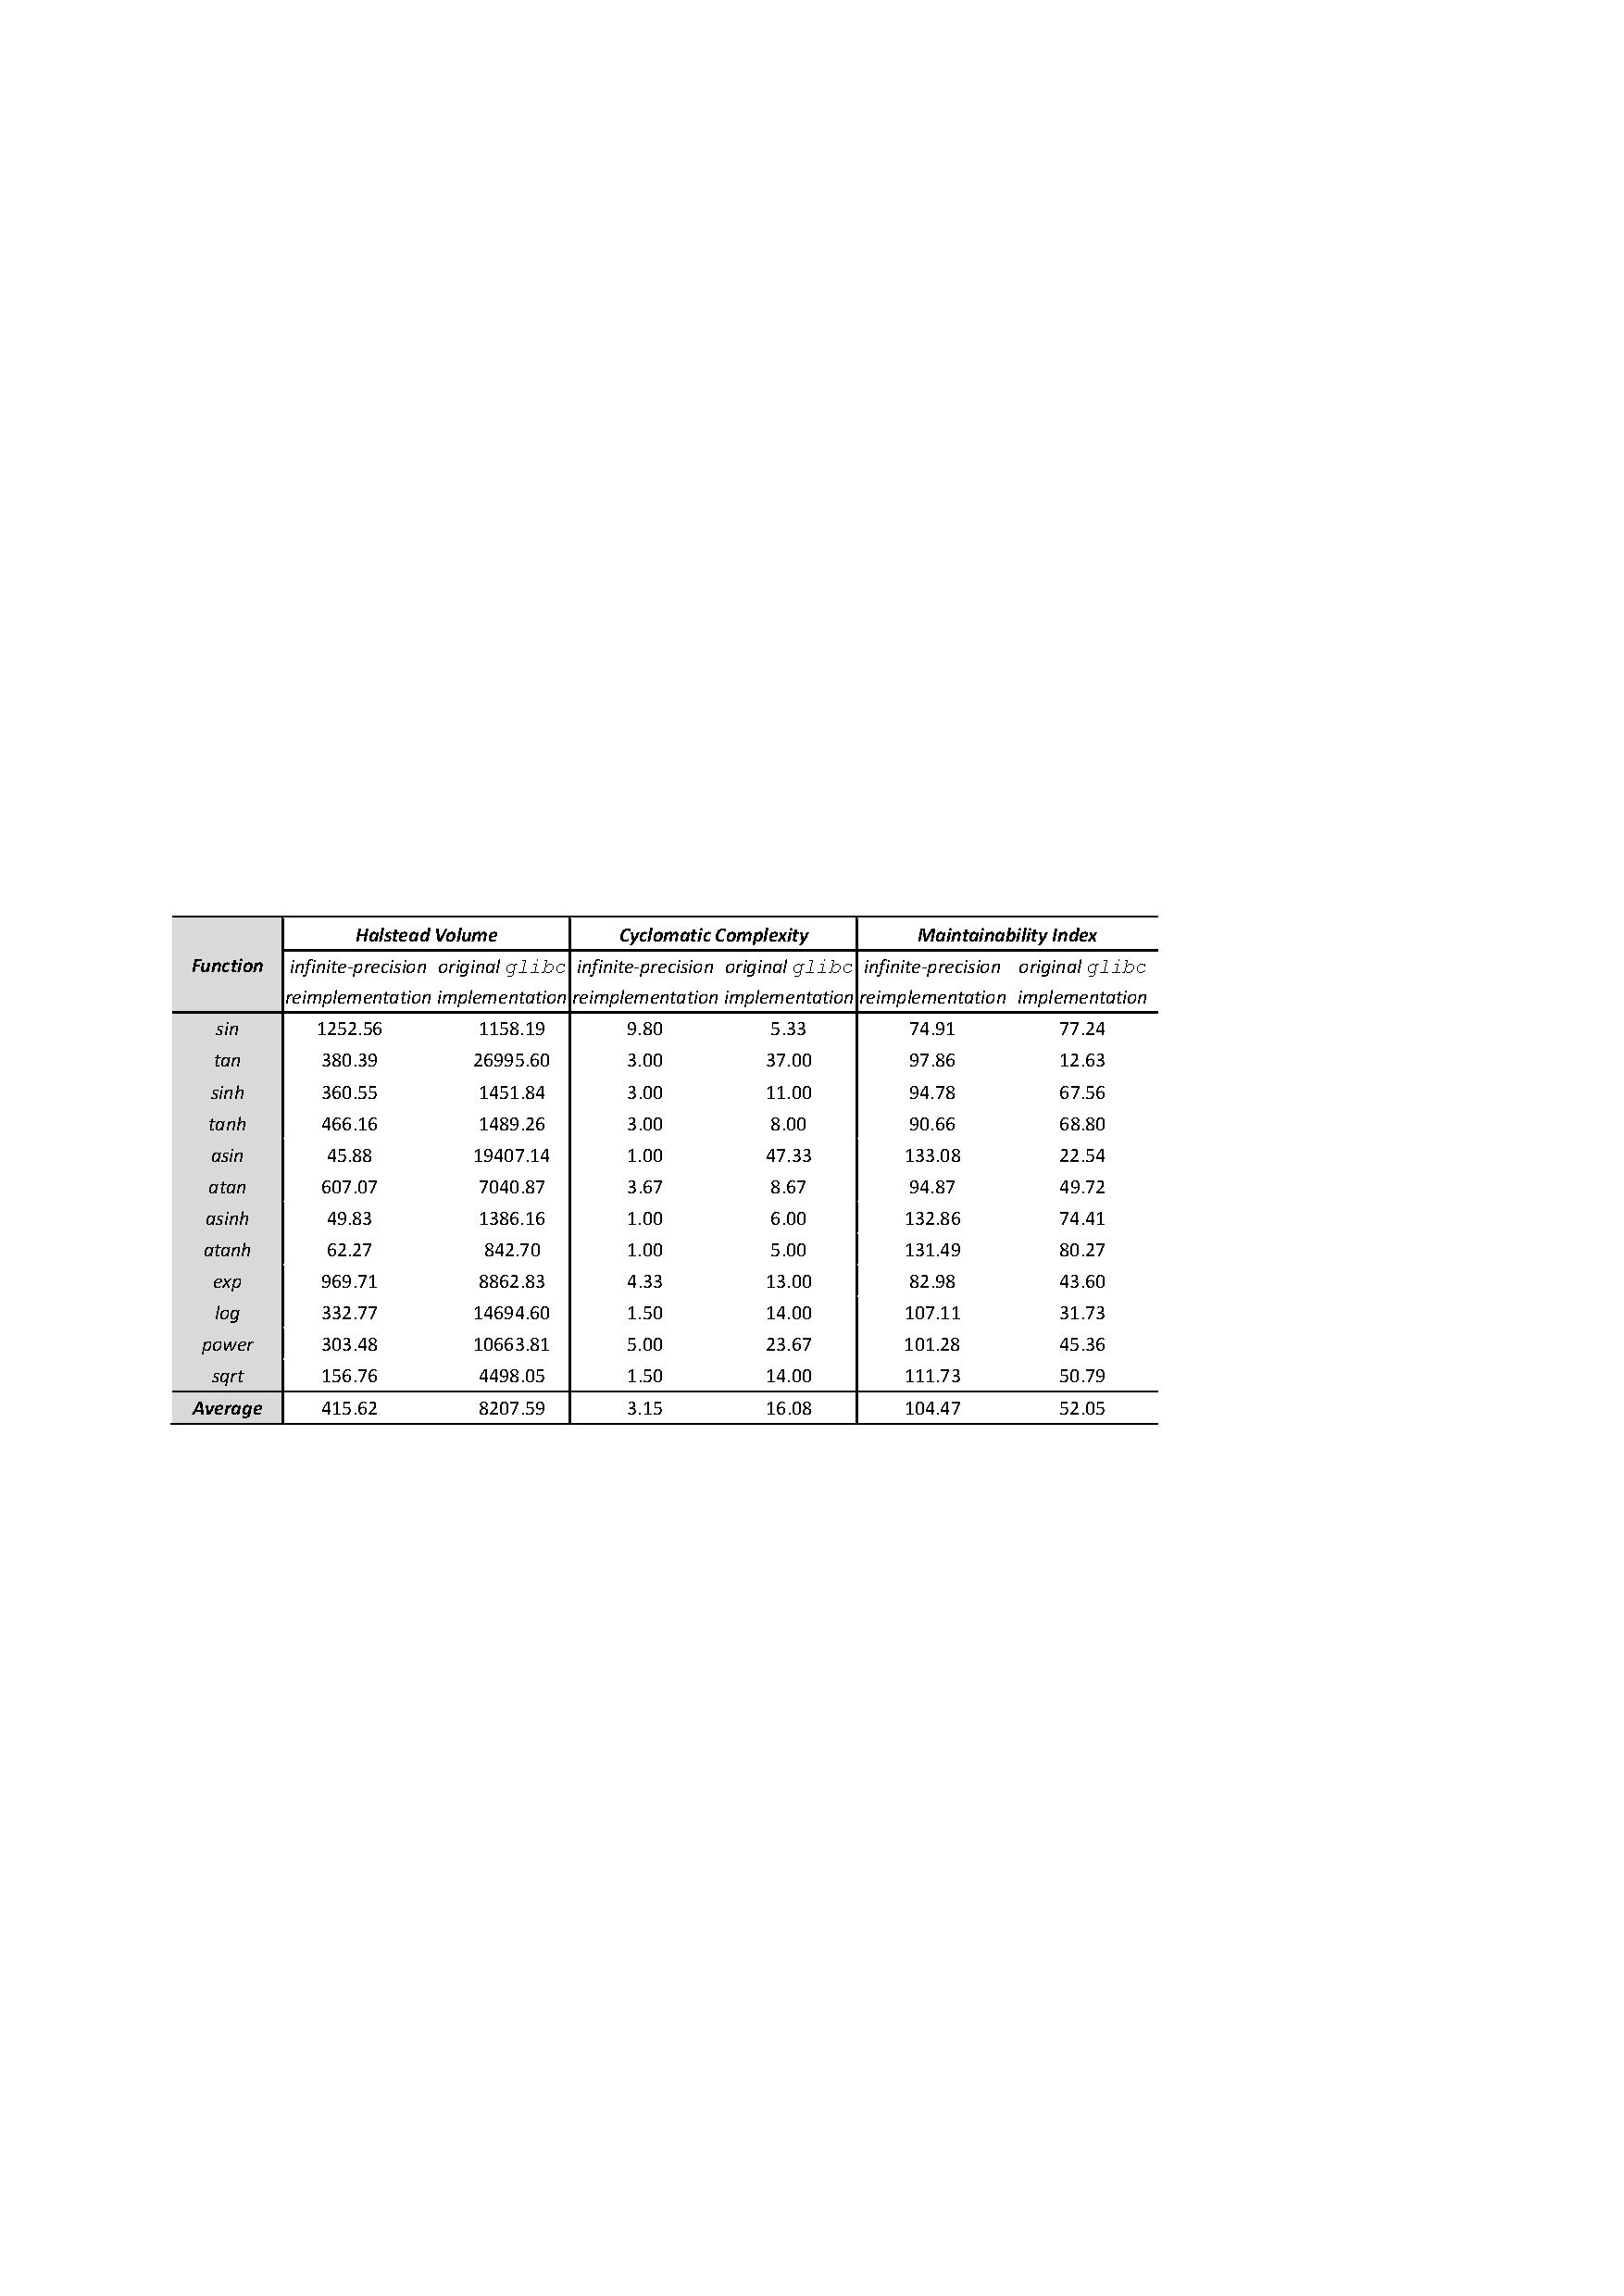
\includegraphics[width=\columnwidth]{fig/EvalTable_ComplexMeasurements.pdf}
    \caption{glibc数学函数在不同实现下各度量指标对比表} \label{fig:complex_measurements}
 \end{table*}

表\ref{fig:complex_measurements}展示了两种不同实现的个度量指标的对比,某些函数使用了大量相同的代码实现,其各项度量指标基本保持一致,因此我们在这里只列举了其中的一个(例如sin函数与cos函数)。从图中我们可以观察到,由于数值计算专家在实现浮点精度的数值计算程序时引入了大量的精度相关的操作,导致glibc的函数实现相比于我们使用任意精度实现的代码复杂了很多。任意精度代码的平均霍尔斯特德复杂度大概只有浮点精度代码的二十分之一,圈复杂度也仅仅只有任意精度代码的五分之一。浮点精度代码的平均可维护性指为104.47,是任意精度代码的两倍左右。从上述实验结果我们可以看出,使用任意精度编写代码,然后使用优化框架进行优化这样的开发数值计算程序的开发方式比直接使用浮点精度代码进行开发能够使程序更加简洁,具有更高的可读性与可维护性。于此同时,程序员即便不具备数值计算专家的专业知识,也能够开发出高效正确的数值计算代码。

\section{本章小结}

在本章中,我们基于上一章节中提到的数值程序的优化方法,实现了一个数值计算程序的优化工具NGOpt,并具体介绍了一些重点的模块,包括基于KLEE符号执行完成的路径提取模块,基于规则模板的随机代数变换引擎等。

随后我们进一步的说明了工具的使用方法,使用工具时各个配置项的具体含义。为了验证我们的工具在对于现实世界中的数值计算程序的优化效果,我们选取了iRRAM高精度数值计算库中的一系列测试程序进行了优化。结果表明,我们的工具能够在不影响程序正确性的情况下极大地提升数值计算程序的运行效率。而后,为了说明我们的工具能够帮助软件开发人员更加轻松地开发高效正确的数值计算代码,我们选取了gblic中部分常用的数学函数,比较了直接的浮点精度实现以及任意精度实现在各个度量指标上的表现,证明了我们的工具的确可以极大提升软件开发人员在开发数值计算程序时的开发效率,同时也能够使得数值计算程序更加易读易维护。